\documentclass[nfss,times,12pt,a4paper]{article}
\usepackage{epsfig}
\usepackage{times}
\usepackage{rotate}
\usepackage{graphicx}

\title{ {\Huge{\bf{ \sc GiGa:} } } \\ 
{ ${\mathcal{GAUDI}}$  Interface for {\it Geant4} Applications }
\\         or  \\ 
{ {\it Geant4} Interface for ${\mathcal{GAUDI}}$ Applications}\footnote{%
The document could be found in {\tt \$GIGAROOT/doc/GiGa.ps}
}  }
\author{ I.Belyaev\footnote{\tt E-mail: Ivan.Belyaev@itep.ru} \\
{\it ITEP (Moscow) } } 
\begin{document}
\maketitle 

\abstract{ 
Proposal for accessing of  {\it Geant4} facilities from 
${\mathcal{GAUDI}}$ framework is discussed. 
This proposal allows the smooth step-by-step transition 
from  stand-alone {\it Geant4} applications into 
applications fully embedded into \linebreak
${\mathcal{GAUDI}}$ 
architecture to be performed. 
The proposed service for communications of 
algorithms within ${\mathcal{GAUDI}}$ framework 
with {\it Geant4} structures allows the usage of {\it Geant4 Tool Kit} 
as a black-box without detailed knowledge of its internal 
features.


\tableofcontents 

\clearpage 
 	
\section     { {\it Simulation}  as a "black-box"  }

{\it Simulation} is an essential part of the  general software 
in modern High Energy Physics. It is foreseen to use 
{\it Geant4 Tool Kit} as the major simulation package  
for the LHC era.  

\subsection { Natural decomposition of {\it Simulation Environment} } 

It is worth to consider any {\it simulation program } 
as sequence of steps, each of them  could be represented 
as the black-box with some well defined input and output data flow.  

For almost each {\it simulation program} it is natural to 
identify the following steps: 	
\begin{itemize} 	
\item {\it Initialisation: }        \\ 
        At this step  {\it simulation program} requires 
        to be provided with some {\it Input Data}: 
        physical properties of all participating 
        components, like 
        particles properties, properties of
        physical processes, description of  
        geometry and materials.            
\item {\it Event Loop     } 
\begin{itemize}	
  \item {\it Event Initialisation } \\ 
          At this step  {\it simulation program} requires 
          to be provided with some {\it input sata} - initial kinematics 
  \item {\it Event Processing     } \\
          At this step simulation program usually neither  
          require to be provided with some {\it input data} 
          nor produce some {\it output data}, but some 
          {\it user action} methods are to be supplied 
          to the {\it simulation program},
          e.g. notorious  {\tt gustep.F} routine 
          in {\tt GEANT3} package.  
  \item {\it Event Finalisation   } \\    
          At this step  {\it simulation program} is ready to provide  
          the {\it user program} with the simulation {\sl output data} 
          - hits, digits and output kinematics - secondary particles. 
\end{itemize} 
\item {\it Finalisation   } 
\end{itemize} 

\subsection  { Communication categories } 

From above sketched rough scheme one could deduce 
that all {\it communications} of {\it user program} 
with {\it simulation environment} could be naturally 
subdivided into 2 categories:

\begin{itemize}
\item {\it Method-like Category:} \\
           Communications from this category 
           are  characterised by dealing mainly with 
           internal structures of {\it simulation program}.
           They do not produce or consume the {\it data}  
           from the outside of the {\it simulation environment}.
           Usually they overwrite some internal default dummy 
           methods from {\it simulation environment}.   
           {\tt gustep.F } could be considered as a typical 
           representative of such category.
\item {\it Stream-like Category:} \\ 
           Communications from this category 
           are  characterised by either producing the  
           {\it data}, which to be used outside of the 
           {\it simulation environment}, like hits, digits, 
           secondary particles, histograms and n-tuples,   
           or they load data flow from the outside 
           of the simulation program, like  particle properties, 
           properties of physical processes and detector description. 
           Usually communications from this category could be easily 
           identified as {\it input streams} or {\it output streams}.
           Routine {\tt guout.F } could be considered as a typical 
           representative of {\it output stream } category and 
           routine {\tt gukine.F } could be considered as a typical 
           representative of {\it input stream } category.
\end{itemize} 
	
Also {\it communications } could be classified into 2 classes:
\begin{itemize} 	
 \item {\it Configuration  Communications:} \\ 
        Such type of communication is used for configuration of the 
        {\it simulation environment} and supplying it with {\it input
        data} which are constant for a some period, sometimes for 
        the whole job  lifetime.  
 \item {\it Event-by-event Communications:} \\ 
        Such type of communication is used on {\it event-by-event basis}
\end{itemize} 

\subsection{ {\sl Communications} with {\it Geant4 Tool Kit} } 

A schematic view of {\sl communications}  with {\it Geant4 Tool Kit } 
is presented on figure~\ref{figOne}. Arrows represent the direction 
of data flows.
 
\begin{figure}[ht] 
\setlength{\unitlength}{1mm} 
\begin{picture}(120,50)
\put(30,0){
\epsfig{file=GiGa_0_m.ps,%
height=50mm,%
bbllx=0pt,bblly=60pt,bburx=590pt,bbury=510pt,clip=}
}
\end{picture} 
\label{figOne} 
\caption{ A schematic view of {\sl communications} with {\it Geant4 Tool Kit}.
Data flow directions are indicated by arrows. }
\end{figure} 


\section     { {\sc GiGa } Service as {\it Simulation Service} } 
	
\subsection  { Why {\it Service} ? } 
Taking into account the rough schemes from section 1, 
and definitions of  ${\mathcal{GAUDI}}$ categories, 
one could easily deduce that the most suitable form 
for embedding the {\it simulation environment} 
into ${\mathcal{GAUDI}}$ framework is {\it Service}. 
 	
Several simple and independent 
${\mathcal{GAUDI}}$ {\it Algorithm}s and {\it Converters} 
could communicate with with {\it Simulation Service} 
suppling it with {\it input data}: detector description, 
particle properties, description of physical processes, 
cut-offs and initial kinematics and retrieving from it the 
{\it output data} in the format of hits and secondaries. 

The service implements two {\it abstract interface}s:
\begin{itemize} 
\item {\it IGiGaSvc interface:}      \\  for {\it event-by-event communication}s 
\item {\it IGiGaSetUpSvc interface:}  \\ for {\it configuration  communication}s 
\end{itemize} 


\subsection  { \it IGiGaSvc      Interface         } 
  
All {\it event-by-event} {\it stream-like communications}  
with {\it simulation environment} defined in {\it IGiGaSvc} 
abstract interface.  This interface is designed to manipulate with
{\it input event data} and {\it output event data}: 
\begin{itemize} 
      \item {\it Input Event Data} are accepted in the form of 
      \begin{itemize}
            \item {\tt G4PrimaryVertex*} \\ 
                  representing the {\it Geant4 primary event record}
            \item {\tt MCVertex*} \\
                  representing the whole event record, starting with {\it primary vertex}
            \item {\tt MCParticle*} \\ 
                  representing the whole event record, starting with {\it primary particle}
      \end{itemize} 
      \item {\it Output Event Data}, retrieved from the {\it Service}  could be of the format:
      \begin{itemize}
            \item {\tt G4Event* } \\
                  provide the access to the whole internal processed event  
            \item {\tt G4HCofThisEvent* } \\
                  provide the access to the all hit collections of the processed event
            \item {\tt CollectionPair* } \\
                  provide the access to the specific hit collection
            \item {\tt G4TrajectoryContainer* } \\
                  provide the access kinematic of secondaries  
      \end{itemize} 
\end{itemize} 


Since all communications with {\it simulation environment} via {\it IGiGaSvc} 
interface are {\it stream-like communications}, the overloaded stream operators are 
considered as main methods in the interface definition: 

\begin{tiny}
\begin{verbatim}
  /////////////////////////////////////////////////////////////////////////////////
  ///                                                                           ///
  virtual IGiGaSvc&   operator <<         ( G4PrimaryVertex  * vertex   ) = 0 ; /// 
  virtual IGiGaSvc&   operator <<         ( const MCVertex   * vertex   ) = 0 ; /// 
  virtual IGiGaSvc&   operator <<         ( const MCParticle * particle ) = 0 ; /// 
  ///                                                                           ///
  /////////////////////////////////////////////////////////////////////////////////
  ///                                                                           ///
  virtual IGiGaSvc& operator >> ( const G4Event*         & event        ) = 0 ; /// 
  virtual IGiGaSvc& operator >> ( G4HCofThisEvent*       & collections  ) = 0 ; /// 
  virtual IGiGaSvc& operator >> ( CollectionPair         & collection   ) = 0 ; ///
  virtual IGiGaSvc& operator >> ( G4TrajectoryContainer* & trajectories ) = 0 ; ///
  ///                                                                           ///
  /////////////////////////////////////////////////////////////////////////////////
\end{verbatim}  
\end{tiny}

In addition to these straightforward definitions, ordinary 
old-fashioned function-like methods are defined:  
\begin{tiny}
\begin{verbatim}
  /////////////////////////////////////////////////////////////////////////////////
  ///                                                                           ///
  virtual StatusCode  addPrimaryKinematics( G4PrimaryVertex  * vertex   ) = 0 ; /// 
  virtual StatusCode  addPrimaryKinematics( const MCVertex   * vertex   ) = 0 ; /// 
  virtual StatusCode  addPrimaryKinematics( const MCParticle * particle ) = 0 ; /// 
  ///                                                                           ///
  /////////////////////////////////////////////////////////////////////////////////
  ///                                                                           ///
  virtual StatusCode retrieveEvent          ( const G4Event*          & ) = 0 ; ///
  virtual StatusCode retrieveHitCollections ( G4HCofThisEvent*        & ) = 0 ; ///
  virtual StatusCode retrieveHitCollection  ( CollectionPair          & ) = 0 ; ///
  virtual StatusCode retrieveTrajectories   ( G4TrajectoryContainer*  & ) = 0 ; ///
  ///                                                                           ///
  /////////////////////////////////////////////////////////////////////////////////
\end{verbatim}  
\end{tiny}

The functionality of these methods almost the same.
The difference belongs to the error handling. In the 
case of errors the operator-like calls throw  
{\tt GiGaException}, while function-like calls return
the {\tt StatusCode::FAILURE}.


\subsection  { \it IGiGaSetUpSvc Interface         }   

All {\it configuration communications} with {\it Simulation Service }
are defined in {\it IGiGaSetUpSvc interface}. 

The interface consists of the following definitions of operator-like calls:
\begin{tiny}
\begin{verbatim}
  /////////////////////////////////////////////////////////////////////////////////
  ///                                                                           /// 
  virtual IGiGaSetUpSvc& operator << ( G4VUserDetectorConstruction   * ) = 0 ;  ///
  virtual IGiGaSetUpSvc& operator << ( G4VPhysicalVolume             * ) = 0 ;  ///
  virtual IGiGaSetUpSvc& operator << ( G4VUserPrimaryGeneratorAction * ) = 0 ;  ///
  virtual IGiGaSetUpSvc& operator << ( G4VUserPhysicsList            * ) = 0 ;  ///
  virtual IGiGaSetUpSvc& operator << ( G4UserRunAction               * ) = 0 ;  ///
  virtual IGiGaSetUpSvc& operator << ( G4UserEventAction             * ) = 0 ;  ///
  virtual IGiGaSetUpSvc& operator << ( G4UserStackingAction          * ) = 0 ;  ///
  virtual IGiGaSetUpSvc& operator << ( G4UserTrackingAction          * ) = 0 ;  ///
  virtual IGiGaSetUpSvc& operator << ( G4UserSteppingAction          * ) = 0 ;  ///
  virtual IGiGaSetUpSvc& operator << ( G4VisManager                  * ) = 0 ;  ///
  ///                                                                           /// 
  /////////////////////////////////////////////////////////////////////////////////
\end{verbatim}  
\end{tiny}

Here the advantage of 
operator-like methods is not so clear and obvious. 

\begin{tiny}
\begin{verbatim}
  /////////////////////////////////////////////////////////////////////////////////
  ///                                                                           /// 
  virtual StatusCode setConstruction ( G4VUserDetectorConstruction   * ) = 0 ;  /// 
  virtual StatusCode setDetector     ( G4VPhysicalVolume             * ) = 0 ;  /// 
  virtual StatusCode setGenerator    ( G4VUserPrimaryGeneratorAction * ) = 0 ;  /// 
  virtual StatusCode setPhysics      ( G4VUserPhysicsList            * ) = 0 ;  /// 
  virtual StatusCode setRunAction    ( G4UserRunAction               * ) = 0 ;  /// 
  virtual StatusCode setEvtAction    ( G4UserEventAction             * ) = 0 ;  /// 
  virtual StatusCode setStacking     ( G4UserStackingAction          * ) = 0 ;  /// 
  virtual StatusCode setTracking     ( G4UserTrackingAction          * ) = 0 ;  /// 
  virtual StatusCode setStepping     ( G4UserSteppingAction          * ) = 0 ;  /// 
  virtual StatusCode setVisManager   ( G4VisManager                  * ) = 0 ;  /// 
  ///                                                                           /// 
  ////////////////////////////////////////////////////////////////////////////////
\end{verbatim}  
\end{tiny}

The functionality of these methods almost the same.
The difference belongs to the error handling. In the 
case of errors the operator-like calls throw  
{\tt GiGaException}, while function-like calls return
the {\tt StatusCode::FAILURE}.


\subsection  { Initial Kinematics }

Primary event record for {\it Geant4} is created  by 
providing of {\sc GiGa} Service via {\it IGiGaSvc} 
interface  with pointers to 
{\tt G4PrimaryVertex},{\tt MCVertex } and/or {\tt MCParticle}
objects. A very complex event could be prepared by 
subsequent calls. 
The call with {\tt NULL} pointer triggers 
the event generation using the instance 
of {\tt G4VUserPrimaryGeneratorAction} class, 
which in this case must be provided to {\sc GiGa} Service 
via {\it IGiGaSetUpSvc interface}. 

\subsection  { Detector Description } 

{\sc GiGa} {\it Service} must be provided with 
detector description either in the form of 
pointer to the "root" object of the type 
{\tt G4VPhysicslVolume} or by 
declaration of the instance of the class 
{\tt G4VUserDetectorConstuction}. Both declarations 
do through {\it IGiGaSetUp interface}.  

\section{ Foreseen {\sc GiGa} Evolution } 
A detailed review on possible schemes of {\sc GiGa} evolution 
are presented in a separate document\footnote{The document could be found at {\tt \$GIGAROOT/doc/GiGaEvolution.ps} }
Here we  report only short extracted snapshots of the foreseen 
{\sc GiGa} evolution of and related stuff. According to described
below  phase classification we are now just in the start of 
Phase~II\footnote{Several steps from Phase~II are already 
performed, but unfortunately they are not tested well enough}.  



\subsection{ Phase I  } 

At this phase we foreseen the 
direct usage of {\sc GiGa} Service 
and some limited number of 
{\it Geant4} classes 
by {\it user}'s  algorithms. 

This case corresponds to a native 
usage of "stand-alone" {\it Geant4} application 
within ${\mathcal{GAUDI}}$ framework. 
{\it User}'s algorithms act like wrappers over 
main program of {\it Geant4}.  
Frankly speaking at very beginning the only 
one profit that ordinary user gets from 
usage {\sc GiGa} Service with respect to 
an ordinary "stand-alone" {\it Geant4} program, 
is the fast and easy access to general and 
technical  ${\mathcal{GAUDI}}$ facilities 
like histogram, code profiling and others.  
 On other side, if one has the working 
{\it Geant4} code, it could be embedded into 
${\mathcal{GAUDI}}$ framework 
using {\sc GiGa} facilities in a straightforward 
way without changing 
any line of codes\footnote{Only the {\tt main() } function is to be removed}. 
   
\subsection{ Phase II  }
 
This phase could be considered as 
{\it "transition phase"}  between Phase~I and Phase~III and 
it could be easily subdivided into some steps:

\begin{enumerate} 
\item 
At this step we enhance the functionality 
of {\sc GiGa} by making possible to extract the 
event record  from ${\mathcal{GAUDI}}$ {\it event store} 
\item 
At this step we enhance the functionality 
of {\sc GiGa} by making possible to get the 
Detector Description by pointing into the root of 
already constructed {\it Geant4} tree 
\item 
At this step we foreseen to implement the automatic
translation of ${\mathcal{GAUDI}}$ Detector 
Description into {\it Geant4} detector description.  
\item 
At this step we foreseen to implement the automatic
creation of {\it Geant4 hits} and {\it sensitive volume}
from their description via XML. A some common 
brainstorming within close collaboration with 
sub-detector groups is necessary for performing of 
this step.    
\item 
At this step we foreseen to automatic
translation of {\it Geant4 hits} into 
${\mathcal{GAUDI}}$ Monte Carlo objects\footnote{Obviously this step could not be done without close collaboration with sub-detector groups}
\item 
At this step we foreseen to automatic
population of ${\mathcal{GAUDI}}$ {\it event store} by information from 
 {\it Geant4 trajectories}\footnote{Communications physics and generator groups are required}
\end{enumerate} 
 
After implementing first two steps 
{\sc GiGa} Service could be considered as {\it "frozen"}, since all other 
steps to Phase~III will not require any change in functionality of {\sc GiGa} Service itself. 

\subsection{ Phase III } 

At this phase no any {\it user}'s algorithm
deals directly with {\sc GiGa } Service and  
{\it Geant4} classes. All knowledge of  
{\it Geant4} will be absorbed by set of specific 
{\it Converters}. This set of specific {\it Converters} 
corresponds to an additional layer in the data flow,  
making the user free from the knowledge
 of {\it Geant4} machinery.    

Being at this phase we could start to think about 
configuration of {\it Geant4} {\it physics list} 
and/or {\it cut-offs} using internal 
${\mathcal{GAUDI}}$ features like 
{\it jobOptions Service} and/or {\it interactive scripting language}. 
Moreover at this stage we foreseen the embedding of  
the essential commands from {\it Geant4} interactive 
{\it user interface} into 
${\mathcal{GAUDI}}$ {\it interactive scripting language}.     

\section     { Summary                             } 

\clearpage 


\section*                     {Appendix~A: \\ {\it Geant4} user classes                    }
\addcontentsline{toc}{section}{Appendix~A: {\it Geant4} user classes                     }

Straightforward communication of user program 
with {\it Geant4 environment} could be represented 
as communications between simulation environments, 
represented by with {\tt G4RunManager} class 
and {\it user program} by set of {\it user classes }.  
{\it User environment} creates these classes, and 
{\it simulation environment} uses them. The sketch is 
presented on figure~\ref{figTwo}.

\begin{figure}[htb] 
\setlength{\unitlength}{1mm} 
\begin{picture}(100,80)
\put(25,0){
\epsfig{file=g4_1.eps,%
height=80mm,%
bbllx=0pt,bblly=480pt,bburx=440pt,bbury=820pt,%
clip=}
}
\end{picture}
\label{figTwo} 
\caption{ Sketch of classes, essential for configuration of {\it Geant4 Tool Kit}} 
\end{figure} 

{\tt G4RunManager} class requires to be provided 
with 3 mandatory classes: 
\begin{itemize} 
 \item {\tt G4VUserDetectorConstruction} 
 \item {\tt G4VUserPhysicsList}
 \item {\tt G4VUserPrimaryGeneratorAction}
\end{itemize} 
In addition {\tt G4RunManager} could be provided with: 
\begin{itemize} 
 \item {\tt G4UserRunAction} 
 \item {\tt G4UserEventAction}
 \item {\tt G4UserStackingAction} 
 \item {\tt G4UserSteppingAction}
 \item {\t G4UserTrackingAction}
\end{itemize} 

The exist also 2 classes, which are to be created explicitly within 
{\it user environment} and which communicate with {\tt G4RunManager} 
in a hidden way:
\begin{itemize}
\item {\tt G4VisManager }  for visualisation 
\item {\tt G4UIsession  }  for interactivity 
\end{itemize}  
	

\section*                     {Appendix~B: \\ Implementation details of {\sc GiGa} Service }
\addcontentsline{toc}{section}{Appendix~B: Implementation details of {\sc GiGa} Service }

Class {\tt GiGaSvc} implements both abstract 
interfaces {\it IGiGaSvc} and {\it IGiGaSetUpSvc}. 
This class is responsible for creation of {\tt GiGaRunManager}, which in turn 
privately inherits from {\tt G4RunManager} class. 
Schematic view is presented in figure~\ref{figThree}.
This implementation prevents the user from  instantiation of 
more then one instance of {\tt GiGaSvc} class.


\begin{figure}[htb] 
\setlength{\unitlength}{1mm} 
\begin{picture}(100,60)
\put(5,0){
\epsfig{file=GiGa_Gen1_m.ps,%
height=60mm,%
bbllx=0pt,bblly=620pt,bburx=400pt,bbury=820pt,%
clip=}
}
\end{picture}
\label{figThree} 
\caption{ Schematic diagram of {\sc GiGa} Service } 
\end{figure} 

The {\sc GiGa} Service implementation contains only 2 essential methods - creation of 
{\tt GiGaRunManager}  and {\tt GiGaKineManager} classes. The latter is used for 
transformation of {\tt MCParticle} and {\tt MCVertex} structures into 
{\tt G4PrimaryVertex} structure and to be replaced in future 
by set of specialised {\it Converter}s. All other methods are just delegation to 
{\tt GiGaRunManager} class. 

{ \tt GiGaRunManager } class is the only non-trivial class in the whole chain. 
It privately inherits from {\tt G4RunManager} class.
The direct communication of user with this class are 
not foreseen. All communications are to be proceed 
only via {\sc GiGa} Service. 

Interface consists of 2 parts. 
\begin{itemize} 
\item Configuration part corresponds to functionality from 
{\it IGiGaSetUpSvc} interface of {\sc GiGa} Service.  
\begin{tiny}
\begin{verbatim}
  /////////////////////////////////////////////////////////////////////////////////
  ///                                                                           ///
  virtual StatusCode declare( G4VUserPrimaryGeneratorAction  * ) ;              /// 
  virtual StatusCode declare( G4VPhysicalVolume              * ) ;              /// 
  virtual StatusCode declare( G4VUserDetectorConstruction    * ) ;              ///
  virtual StatusCode declare( G4VUserPhysicsList             * ) ;              /// 
  virtual StatusCode declare( G4UserRunAction                * ) ;              /// 
  virtual StatusCode declare( G4UserEventAction              * ) ;              ///
  virtual StatusCode declare( G4UserStackingAction           * ) ;              /// 
  virtual StatusCode declare( G4UserSteppingAction           * ) ;              ///
  virtual StatusCode declare( G4UserTrackingAction           * ) ;              ///
  virtual StatusCode declare( G4VisManager                   * ) ;              ///
  ///                                                                           ///
  /////////////////////////////////////////////////////////////////////////////////
\end{verbatim}  
\end{tiny}
\item Event management part corresponds to functionality from 
{\it IGiGaSvc} interface of {\sc GiGa} Service.  
\begin{tiny}
\begin{verbatim}
  /////////////////////////////////////////////////////////////////////////////////
  ///                                                                           ///
  virtual StatusCode  prepareTheEvent ( G4PrimaryVertex    * vertex = 0 ) ;     ///
  virtual StatusCode  processTheEvent (                                 ) ;     /// 
  virtual StatusCode  retrieveTheEvent( const G4Event      *& event     ) ;     /// 
  ///                                                                           ///
  /////////////////////////////////////////////////////////////////////////////////
\end{verbatim}  
\end{tiny}
\end{itemize} 

All other methods are purely internal and 
irrelevant for external user, thats why all 
of them are protected or private. 

Internally {\tt GiGaRunManager} acts as {\it state machine}.
Each state could be represented as {\it "4-bit word"}:
\begin{itemize}
\item {\it "Kernel Is Initialised" } 
\item {\it "Run    Is Initialised" } 
\item {\it "Event  Is Prepared"    } 
\item {\it "Event  Is Processed"   } 
\end{itemize}
   
Initial state of {\tt GiGaRunManager} corresponds to the all flags are switched off. 

Each communication with configuration part of interface
resets this 4-bit state word to zero. 

Action of each method from event management 
part depends on the concrete current state of {\it GiGaRunManager}. 
\begin{itemize}
      \item {\tt retrieveTheEvent(const G4Event*\& event)} \\  
              If flag {\it "Event Is Processed"} is not activated, 
                         this method forces the processing of the event  by {\tt processTheEvent} method.
        Then if flag {\it "Event Is Processed"} is activated 
                         the method retrieves the current {\tt G4Event*} object, otherwise it fails.
         Method makes sure that the flag {\it "Event Is Processed"} is activated in the case of success.  
      \item {\tt processTheEvent()}\\ 
              If flag {\it "Event Is Processed"} is activated,  
                  the method switched it off and delete the current event. 
              Then if flag {\it "Event Is Prepared"} is not activated, 
                 this method forces the preparation of the event  by {\tt prepareTheEvent(0)} method.
              Then if flag {\it "Event Is Prepared"} is activated 
                         the method start the actual precessing of event, otherwise it fails.
              Method makes sure that the flag {\it "Event Is Processed"} is activated in the case of success.  
      \item {\tt prepareTheEvent( G4PrimaryVertex* vertex = 0 )} \\ 
              If flag {\it "Event Is Processed"} is activated,  
                  the method switched it off and delete the current event. 
              If flag {\it "Event Is Prepared" } is activated 
                  the method add the {\tt vertex} to the current primary 
                event record\footnote{ If {\tt vertex} is {\tt NULL} a new event would be generated using 
              {\it G4VUserPrimaryGeneratorAction} and added to the current one}
              If flag {\it "Event Is Prepared"} is not activated, 
              method starts the real event preparation. Real Event preparation could be possible only if 
flag {\it "Run Is Initialised"} is activated, overwise method forced the run initialisation. 
 If flag {\it "Run Is Initialises"} is activated, a new event is created and {\tt vertex} is added to primary 
 event record.      
              Method makes sure that the flag {\it "Event Is Prepared"} is activated in the case of success.  
\end{itemize}    


\section*                     {Appendix~C: \\ {\sc GiGa} Examples }
\addcontentsline{toc}{section}{Appendix~C: {\sc GiGa} Examples }


A set of examples of usage of {\sc GiGa} Service is prepared.
This set corresponds to a usage of {\sc GiGa} Service for 
the Phase~I. All six standard novice examples from 
{\it Geant4 Tool Kit} distribution are configured to work 
within ${\mathcal{GAUDI}}$ framework. 


\end{document} 















